%TODO: provide your details here.

\begin{frame}
    \frametitle{About Your Fellows}
    \begin{itemize}
        \item Hi there! We are \textcolor{red}{\textbf{Hamza}} {and }\textcolor{red}{\textbf{Fouz}}.
        \item We are Associate Students at ITU.
    \end{itemize}
\end{frame}




\begin{frame}
    \frametitle{Asymptotic Notations}
    \begin{itemize}
        \item\textcolor{black}{Asymptotic Notations}
        \vspace{0.3cm}
        \begin{itemize}
            \item There are three rules behind this idea.
        \end{itemize}
    \end{itemize}
\end{frame}


\begin{frame}
    \frametitle{Rule 1}
      \begin{block}{\textcolor{red}{Rule 1: We take estimations of runtime in terms of bounds.}}
        - Upper bound \\
        - Lower bound \\
        - Tight bound
    \end{block}

    \bigskip % Adds a good amount of space before content

    \begin{itemize}
        \item \textbf{Upper Bound:} \textit{O (Big Oh)}

        \medskip % Adds some space before the nested list

        \begin{itemize}
            \item \textit{$T(n) \leq F(n)$.}
        \end{itemize}

        \vspace{0.2cm}
        \item \textbf{Lower Bound:} \textit{$\Omega$ (Big Omega)}
        \medskip % Adds some space before the nested list
         \begin{itemize}
            \item \textit{$T(n) \geq g(n)$.}
        \end{itemize}


          \vspace{0.2cm}
        \item \textbf{Tight Bound:} \textit{$\Theta$ (Big Theta)}
        \medskip % Adds some space before the nested list
         \begin{itemize}
            \item \textit{$T(n) \geq F(n)$ \& $T(n) \leq F(n)$}
        \end{itemize}

        \vspace{0.2cm}
        \item Where \textit{F \& G} are functions of size N.
    \end{itemize}

    \bigskip % Adds space at the bottom for better layout
\end{frame}


\begin{frame}
    \frametitle{Rule 1}
    \vspace{0.3cm} % Adds spacing for better visual appearance
    \begin{block}
          {For every string input function, the size is the length of that string. Makes sense right?}
    \end{block}
  
    \vspace{0.3cm}
    \begin{itemize}
        \item \textbf{Problem:} \textcolor{red}{If the input is an integer. What will be the size?}
        \vspace{0.3cm} % Adds spacing between items
        \begin{itemize}
            \item \textcolor{black}{Always remember, in e.g., \textit{F(n)}, \textbf{n} is the size for arrays or strings, but for an integer input, the size is O(log n).}
            \item Therefore, we take the number of bits required to display this number as the size. \textit{( Log(n) )}
        \end{itemize}
    \end{itemize}
    \vspace{0.5cm} % Adds spacing at the bottom of the slide for a clean look
\end{frame}


\begin{frame}
    \frametitle{Rule 1}
    \begin{block}{\textcolor{red}{Example:}}
          Mystery(p): \\
        - if $p < 2$: \\
        -  \quad  return 1 \\
        - else: \\
        -   \quad return 1 + Mystery(sqrt(p)) \\
    \end{block}
    \vspace{0.2cm}
    Input Size of this function will be \textit{Log(p)}.
    
\end{frame}

\begin{frame}
    \frametitle{Rule 2}
    \vspace{0.3cm} % Adds spacing for better visual appearance
     \begin{block}{\textcolor{red}{Rule 2: Small Inputs are irrelevant.}}
     When someone gives us a bound on a function, we only need to make sure the bound is valid on a really large n.
    \end{block}
    \vspace{0.2cm}
   \item \textcolor{red}{How Large is really large?} \\
   \vspace{0.2cm}
   As large as you want! \\
   \item Choose a minimum input size n_0.  \\
   \vspace{0.2cm}
   \item \textbf{Upper Bound:} \\
   \vspace{0.2cm}
   \quad \textit{T(n) \leq F(n)} \quad  \forall n > n_0
   
    \vspace{0.5cm} % Adds spacing at the bottom of the slide for a clean look
\end{frame}

\begin{frame}
    \frametitle{Rule 2}
    \vspace{0.3cm} % Adds spacing for better visual appearance
    \begin{block}{\textcolor{red}{Why is that?}}
    \vspace{0.2cm}
    It is because functions can be messy and to actually know what is going on we need a wider picture of it. For example, if we take two graphs, one of x + 1 and one of log x, the graph of x + 1 will dominate it. Now if we multiply log x with a large number like fifty thousand, and take cube of log x, visually it will feel as if the graph of x + 1 is being dominated, but that is not true as there is a point where x+1 will cut log x graph and increase at a greater rate. This is because x + 1 is a linear graph and log x grows much more slowly.
    \end{block}
\end{frame}


\begin{frame}{Graphs}
    \begin{figure}
        \centering
        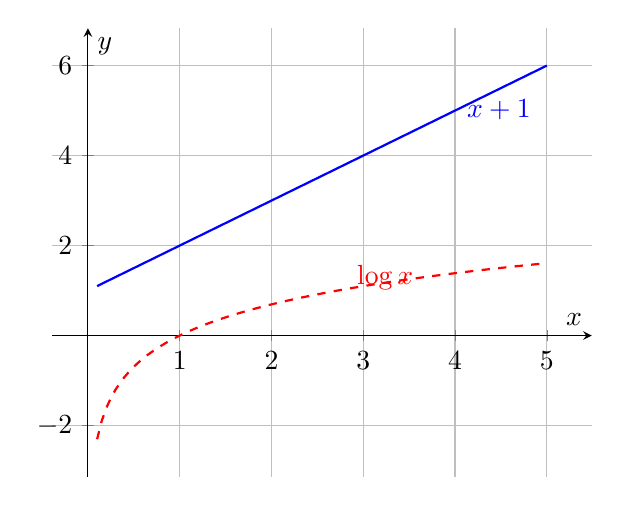
\begin{tikzpicture}
            \begin{axis}[
                xlabel={$x$},
                ylabel={$y$},
                axis lines=middle,
                enlargelimits=true,
                legend pos=north west,
                grid=major,
                domain=0.1:5, % Define x range
                samples=100
            ]
                \addplot[blue, thick] {x+1} node[pos=0.8, anchor=west] {$x+1$};
                \addplot[red, thick, dashed] {ln(x)} node[pos=0.8, anchor=east] {$\log x$};
            \end{axis}
        \end{tikzpicture}
        \caption{Graph of \textbf{\( x+1 \) and \( \log x \)}}
    \end{figure}
\end{frame}






\begin{frame}{Graphs}
    \begin{figure}
        \centering
        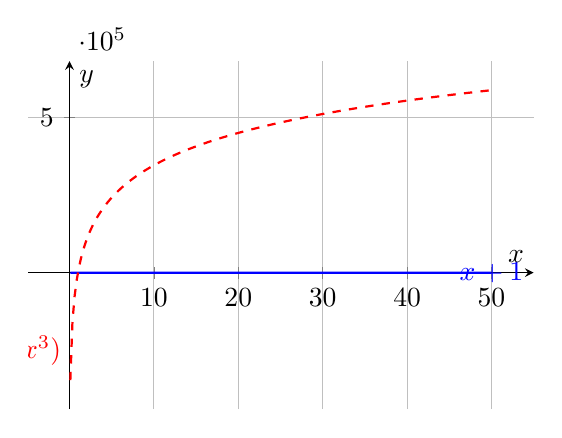
\begin{tikzpicture}
            \begin{axis}[
                width=8cm, height=6cm, % Adjust graph size
                xlabel={$x$},
                ylabel={$y$},
                axis lines=middle,
                enlargelimits=true,
                legend pos=north west,
                grid=major,
                domain=0.1:50, % x should be > 0 for log function
                samples=200
            ]
                % Corrected x+1 plot
                \addplot[blue, thick] {x+1} node[pos=0.9, anchor=west] {\textcolor{blue}{$x+1$}};

                % Corrected log function (log base e)
                \addplot[red, thick, dashed] {50000 * 3 * ln(x)} node[pos=0.1, anchor=east] {\textcolor{red}{$50000 \cdot \log(x^3)$}};
            \end{axis}
        \end{tikzpicture}
        \caption{Graph of \textbf{\( x+1 \) and \( 50000 \cdot \log(x^3) \)}}
    \end{figure}
\end{frame}

\begin{frame}{Graphs}
    \begin{figure}
        \centering
        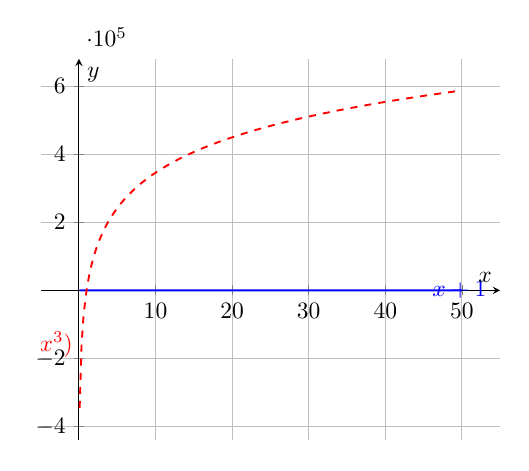
\begin{tikzpicture}[scale=0.85]
            \begin{axis}[
                xlabel={$x$},
                ylabel={$y$},
                axis lines=middle,
                enlargelimits=true,
                legend pos=north west,
                grid=major,
                domain=0.1:50, % Wider view of x range
                samples=200
            ]
                  % Corrected x+1 plot
                \addplot[blue, thick] {x+1} node[pos=0.9, anchor=west] {\textcolor{blue}{$x+1$}};
                
                \addplot[red, thick, dashed] {50000 * ln(x^3)} node[pos=0.2, anchor=east] {\textcolor{red}{$50000 \cdot \log(x^3)$}};
            \end{axis}
        \end{tikzpicture}
        \caption{Graph of \textbf{\( x+1 \) and \( 50000 \cdot \log(x^3) \)} in a wider view}
    \end{figure}
    \begin{itemize}
        \item \centering \textcolor{blue}{\textbf{We can see that the \( x+1 \) graph eventually intersects the \( 50000 \cdot \log(x^3) \) graph.}}
    \end{itemize}
    
\end{frame}




\begin{frame}
    \frametitle{Rule 3}
    \vspace{0.3cm} % Adds spacing for better visual appearance
    \begin{block}{\textcolor{red}{Rule 3: Constants do not matter in asymptotics!}}
    \vspace{0.2cm}
    - If \textit{T(n)} is upper bounded by \textit{F(n)} \\
    - 2 * \textit{T(n)} should also be upper bounded by \textit{F(n)} \\
    - 100 * \textit{T(n)} should also be upper bounded by \textit{F(n)}
    \end{block}
    \vspace{0.2cm}
    This is achieved by allowing a constant to be multiplied with \textit{F(n)} when trying to upper bound \textit{T(n)}.\\
    \vspace{0.3cm}
    \textcolor{blue}{\text{For some } $c>0$, \textit{T(n)} \leq c \cdot \textit{F(n)}, \text{ for } n > n_0}
\end{frame}

\begin{frame}
    \frametitle{Examples}
    \vspace{0.3cm}
    \textbf{Example 1:} Let $T(n) = O(g(n))$ \\
    This implies there exists a constant $c$ such that:
    \[ T(n) \leq c g(n) \]
    
    \textbf{Example 2:} Algorithm Complexity
    \begin{itemize}
        \item Algo 0: Time Complexity = $T(n)$
        \item Algo 1: Loop from $i = 1$ to $100$ \newline
        $\Rightarrow$ Still $O(T(n))$, since constant factors don't matter
        \item Algo 2:
        \begin{itemize}
            \item Loop from $i = 1$ to $10^6$ \newline
            $\Rightarrow O(T(n))$, as it remains bounded by a constant multiple
            \item Loop from $i = 1$ to $n$ \newline
            $\Rightarrow O(n T(n))$, since it scales with $n$
        \end{itemize}
    \end{itemize}
\end{frame}

\begin{frame}
    \frametitle{Conclusion}
    \begin{block}{\textcolor{black}{}}
        \item Therefore, based on these three rules, we have defined that \textit{T(n)} is Big O of \textit{F(n)}, \textit{T(n)} = \textit{0(F(n))}, whenever we can find a constant so that \textit{T(n)} \leq c * \textit{F(n)} , for \ really \ large \ values \ of \ n.
    \end{block}

    
\end{frame}

\begin{frame}
    \frametitle{Quick Sort}
    In  Quick sort we use ranks of each element in an array or list to sort them.
    \begin{itemize}
        \item\textbf{\textcolor{black}{What is the Rank problem:}}
        \begin{itemize}
            \item Rank means the position of an element in a sorted array/list.
            \vspace{0.2cm}
            \item Therefore, one easy way of finding the rank is by first sorting the array, and then using index to find the element's rank.
            \vspace{0.2cm}
            \item Another way is to compare the element with all other elements and count the ones smaller. This is efficient as it is in \textit{O(n)}.
            
        \end{itemize}
    \end{itemize}
\end{frame}




\begin{frame}
    \frametitle{The Rank Problem}
    \begin{itemize}
        \item \textbf{Problem Statement:} 
        \begin{itemize}
            \item Given: Array A (unsorted, distinct elements)
            \item Input: Index i
            \item Goal: Find position of A[i] in sorted version of A
        \end{itemize}
        \vspace{0.3cm}
        \item \textbf{Definition:} 
        \begin{itemize}
            \item Rank(A, i) = Position of A[i] in sorted array
            \item Equivalent to counting elements smaller than A[i]
        \end{itemize}
    \end{itemize}
\end{frame}

\begin{frame}
    \frametitle{Rank Algorithm}
    \begin{block}{Algorithm: Rank(A, i)}
        \begin{enumerate}
            \item Let count = 0
            \item For each j ≠ i in array A:
                \begin{itemize}
                    \item If A[j] < A[i], increment count
                \end{itemize}
            \item Return count + 1 (the rank)
        \end{enumerate}
    \end{block}
    
    \begin{alertblock}{Mathematical Representation}
        Let L = \{A[j] < A[i]\}
        \[
        \text{Rank(A, i)} = |L| + 1
        \]
        where |L| is the number of elements smaller than A[i]
    \end{alertblock}
\end{frame}

\begin{frame}
    \frametitle{Time Complexity Analysis}
    \begin{itemize}
        \item \textbf{Algorithm Cost:}
        \begin{itemize}
            \item Need to compare A[i] with all other elements
            \item Total comparisons = n - 1
            \item Time Complexity: \textcolor{blue}{O(n)}
        \end{itemize}
        \vspace{0.3cm}
        \item \textbf{Key Points:}
        \begin{itemize}
            \item Linear time algorithm
            \item No need to sort the entire array
            \item Direct comparison approach
        \end{itemize}
    \end{itemize}
\end{frame}



\begin{frame}
    \frametitle{Quick Sort}
    \begin{block}{\textcolor{red}{Our Own Version of Quick Sort:}}
     \texttt{
        QS1(A) \{ \\
        \quad B = [ ] \\
        \quad for i = 0 to $|A| - 1$ \\
        \quad x = rank(A,i) \\
        \quad B[x] = A[i]\\ 
        \quad return B\\
        \}
        }
    \end{block}
It compares each element with every other element. Therefore, the complexity of this function is \(\mathcal{O}(n^2)\). \\
\vspace{0.3cm}
\textcolor{red}{We can do better!}
\end{frame}


\begin{frame}
    \frametitle{Quick Sort Example}
    \begin{block}{Initial Array}
        [5, 9, 7, 0, -15, 4, 19]
    \end{block}
    
    \begin{block}{Step 1: Choosing Pivot}
        \begin{itemize}
            \item Choose 5 as pivot
            \item Partition array into:
            \begin{itemize}
                \item Left (smaller): [0, -15, 4]
                \item Pivot: [5]
                \item Right (larger): [9, 7, 19]
            \end{itemize}
        \end{itemize}
    \end{block}
\end{frame}

\begin{frame}
    \frametitle{Quick Sort Example (continued)}
    \begin{block}{Step 2: Recursive Partitioning}
        Left side: [0, -15, 4]
        \begin{itemize}
            \item Choose 0 as pivot
            \item Left: [-15]
            \item Pivot: [0]
            \item Right: [4]
        \end{itemize}
        
        Right side: [9, 7, 19]
        \begin{itemize}
            \item Choose 9 as pivot
            \item Left: [7]
            \item Pivot: [9]
            \item Right: [19]
        \end{itemize}
    \end{block}
\end{frame}


\begin{frame}
    \frametitle{Quick Sort Example (Final)}
    \begin{block}{Final Result}
        \begin{itemize}
            \item Combining all partitions:
            \[ [-15] \rightarrow [0] \rightarrow [4] \rightarrow [5] \rightarrow [7] \rightarrow [9] \rightarrow [19] \]
        \end{itemize}
    \end{block}
    
     \begin{alertblock}{Key Observations}
        \begin{itemize}
            \item Each partition divides the problem into smaller sub problems
            \item Elements are naturally sorted during the partitioning process
            \item More efficient than comparing every element with every other element
            \item \textbf{Mathematical Property:}
            \[ \forall  start \in S, \forall  end \in L: \text{rank}(s) < \text{rank}(l) \implies s < l \]
            where S is the set of smaller elements and L is the set of larger elements
        \end{itemize}
    \end{alertblock}
\end{frame}


\begin{frame}
    \frametitle{Improvised Quick Sort complexity}
    \begin{itemize}
        \item This function uses extra memory as we create separate lists.\\
        \vspace{0.2cm}
        \item Best case we get almost equal lengths of both lists so due to recursion it becomes \textit{O(nlogn)}.\\
        \vspace{0.2cm}
        \item In the worst case, all the elements except one could be on one side and therefore,every element will be compared. So complexity would be \(\mathcal{O}(n^2)\). \\
        \vspace{0.3cm}
        \textcolor{red}{Is there a better approach with better worst case complexity and is in place?} \\
        \vspace{0.2cm}
        YES!
    \end{itemize}
    
\end{frame}


\begin{frame}
    \frametitle{Improvising}
         \texttt{
        QS2(A) \{ \\
        \quad if $|A| \leq 1$ \\
        \quad return A \\
        \quad B = [ ] \\
        \quad S = \{ A$_i$ $|$ A$_i < $ A[0] \} \\
        \quad L = \{ A$_i$ $|$ A$_i > $ A[0] \} \\
        \quad NL = QS2(L) \\
        \quad NS = QS2(S) \\
        \quad B = [ NS, A[0], NL ] \\
        \quad return B \\
        \} \\
        }
        \vspace{0.3cm}
        \textcolor{red}{We do not want to use extra memory at first so it becomes an in place algorithm.}
\end{frame}


\begin{frame}
    \frametitle{Actual Quick Sort}
    
    \textbf{Initial Array:}
    \[
    [\mathbf{5}, 9, 7, 0, -15, 4, 19]
    \]
    Pivot: 5
    
    
    \vspace{0.3cm}
    \textbf{Step 1:} compare 5 with 9. As it is lesser we swap 9 with last element and recursively call without 9.
    
    \[
    [\mathbf{5}, 19, 7, 0, -15, 4, \mathbf{9}]
    \]
     \textbf{Step 2:} compare 5 with 19. As it is lesser we swap 9 with new last element and recursively call without 19,9.
    \[
    [\mathbf{5}, 4, 7, 0, -15, 19, 9]
    \]
 
    \textbf{Step 3:} We compare 5 with 4 and as 4 is lesser we swap with 5 and recursively call without 4
    \[
    [4, \mathbf{5}, 7, 0, -15, 19, 9]
    \]

\end{frame}



\begin{frame}
    \frametitle{Actual Quick Sort}
     \[
    [4, \mathbf{5}, 7, 0, -15, 19, 9]
    \]
    \textbf{Step 4:} We compare 5 with 7 and as 7 is greater we swap with last element which is -15.
    \[
    [4, \mathbf{5}, -15, 0, 7, 19, 9]
    \]
     \textbf{Step 5:} We compare 5 with -15 and as -15 is lesser we swap with 5 and recursively call without -15.
      \[
    [4, -15, \mathbf{5}, 0, 7, 19, 9]
    \]
    Similarly with zero: \\
     \[
    [4, -15, 0, \mathbf{5}, 7, 19, 9]
    \]
    Now only one element is left so return call would be made and we can see that the pivot is at it's correct position. This is only one iteration. Two recursive calls will be made on each side of the pivot until the base case is reached and whole list is then sorted.\\
       \vspace{0.3cm}
    \textcolor{blue}{\textbf{In-Place Algorithm:} Does not allocate more than constant space.}

\end{frame}

\begin{frame}
    \frametitle{QS2 Algorithm: In-Place Quick Sort}
    \begin{itemize}
        \item \textbf{QS2(A, x, y)} is an in-place variant of Quick Sort.
        \item It does not allocate more than \( O(1) \) extra memory.
        \item  Before executing QS2, shuffle the array \( A \) to ensure randomness.
    \end{itemize}
\end{frame}



\begin{frame}
    \frametitle{In-Place QuickSort}
    \begin{block}{\textcolor{red}{QS2: In-Place QuickSort}}
        \texttt{
        def QS2(A, start, end): \\
        \quad if end < start + 1: \\
        \quad \quad return A \\
        \quad i, j = start + 1, end + 1 \\
        \quad p = A[i + 1] \\
        \\
        \quad while i < j - 2: \\
        \quad \quad if A[i + 2] <= A[i + 1]: \\
        \quad \quad \quad i += 1 \\
        \quad \quad if A[i + 2] > A[i + 1]: \\
        \quad \quad \quad A[i + 2], A[j - 1] = A[j - 1], A[i + 2] \\
        \quad \quad \quad j -= 1 \\
        \\
        \quad QS2(A, start, i) \\
        \quad QS2(A, j, end) \\
        \\
        \quad return A
        }
    \end{block}
\end{frame}


\begin{frame}
    \frametitle{Understanding Time Complexity Recurrence}
    \begin{itemize}
        \item The time complexity of QS2:
        \begin{itemize}
            \item \textbf{Worst-case:} \( O(n^2) \) (occurs when the pivot selection is poor).
            \item \textbf{Best-case:} \( O(n \log n) \) (occurs when partitions are balanced).
            \item \textbf{Average-case:} \( O(n \log n) \) (expected performance over random inputs).
        \end{itemize}
        
        \item The recurrence relation for QS2 is given by:
        \[
        T(n) = aT(n/b) + f(n)
        \]
        \item If we assume a randomized pivot selection:
        \[
        a_1, a_2, a_3, \dots\dots, a_{n-3}, a_{n-2}, a_{n-1}, a_n
        \]
        \item The pivot is expected to lie between \( \frac{n}{4} \) and \( \frac{3n}{4} \), leading to more balanced partitions.
        \item If \( |S| < \frac{n}{4} \) or \( |L| < \frac{n}{4} \), we may need to recompute the partition.
    \end{itemize}
\end{frame}

\begin{frame}
    \frametitle{Randomized Quick Sort: Expected Runtime}
    \begin{itemize}
        \item Randomized Quick Sort improves partitioning by choosing a random pivot, reducing the likelihood of worst-case behavior.
        \item The recursive relation for randomized Quick Sort is:
        \[
        T(n) = T(|L|) + T(n - |L| - 1) + cn
        \]
        \item Expected time complexity analysis:
        \[
        E(T(n)) = 2cn + E(T(|L|)) + E(T(n - |L| - 1)) \leq c2n
        \]
        \item By maintaining a balanced partition, we can ensure an average-case complexity of \( O(n \log n) \).
    \end{itemize}
\end{frame}

\begin{frame}
    \frametitle{Quick Sort Partitioning Visualization}
    
    \begin{figure}
        \centering
        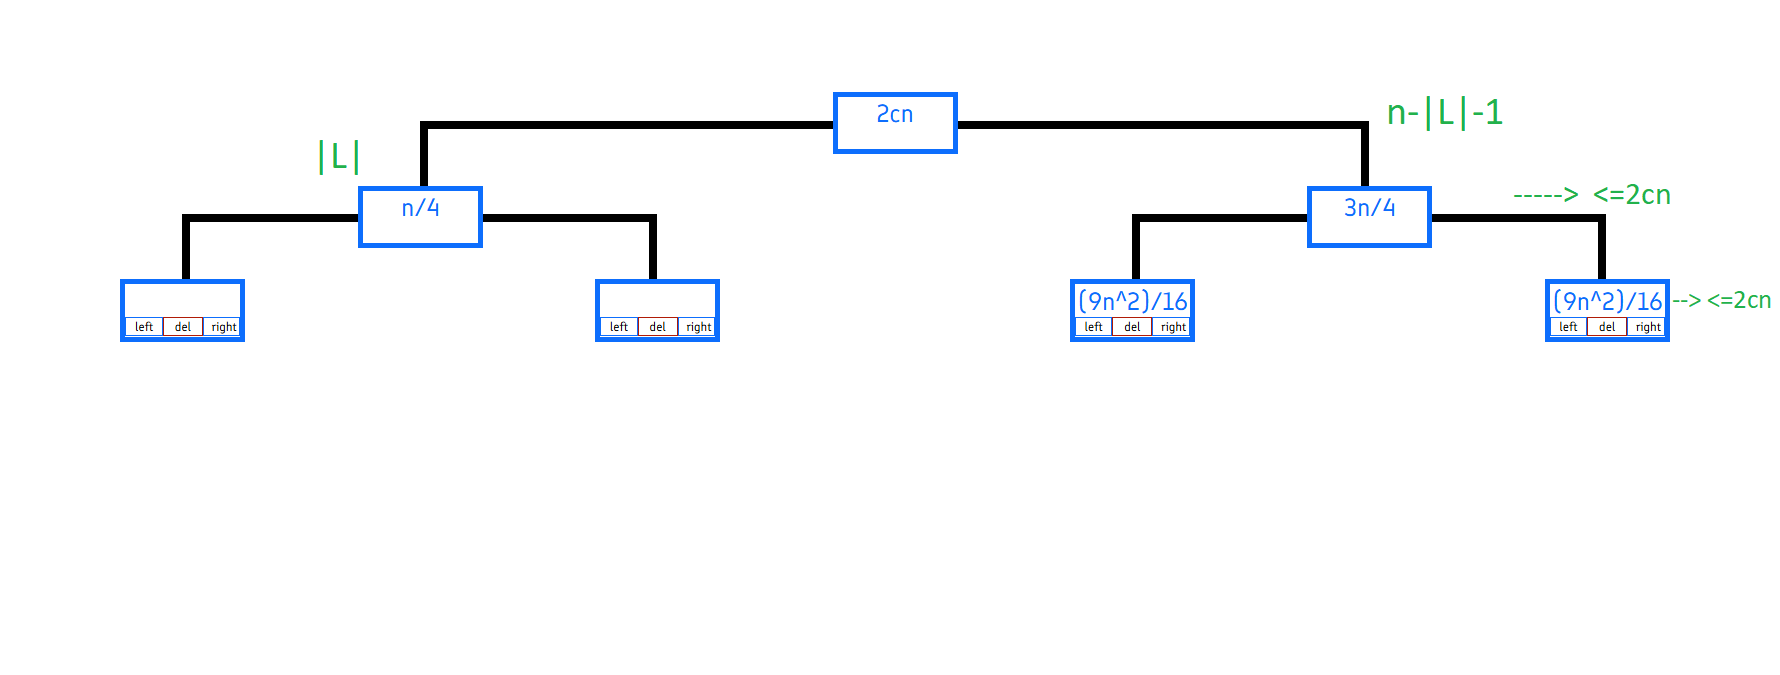
\includegraphics[width=0.7\linewidth]{figures/general/tree.png}
        \caption{Recursive Tree of Quick Sort }
    \end{figure}
    
    \begin{itemize}
        \item The pivot is chosen, and the array is divided into two subarrays.
        \item Elements smaller than the pivot move to the left; larger ones move to the right.
        \item The process repeats recursively until the array is sorted.
    \end{itemize}
\end{frame}



\begin{frame}
    \frametitle{Quick Sort: Longest Branch and Expected Complexity}
    
    \begin{itemize}
        \item The \textbf{right-side} branch in the Quick Sort recursion tree is the \textbf{longest branch.}
        \item The recursion reaches \textbf{1} when \( k \approx \log n \).
        \item Given the inequality:
        \[
        (3/4)^kn \leq 1
        \]
        \item Solving for \( k \):
        \[
        k \log(3/4) + \log n \leq 1
        \]
        \[
        k \log(3/4) \geq \log n - 1
        \]
        \[
        k \approx \log n
        \]
        \item Since \( k \approx \log n \), the expected time complexity for Quick Sort is:
        \[
        E(T(n)) = O(n \log n)
        \]
    \end{itemize}

\end{frame}




\begin{frame}
    \begin{center}
        \vspace*{1cm}  % Add some vertical space at the top
        {\Large \textcolor{red}{\textbf{Algorithms, Design \& Analysis}}}
        
        \vspace{0.5cm}  % Space between title and subtitle
        {\textcolor{red}{\large Lecture 06: }\textcolor{blue}{\textbf{Quick Sort And Merge Sort}}}
        
        \vspace{1cm}  % Space below subtitle
    \end{center}
\end{frame}






\begin{frame}
    \frametitle{Quick Sort Recap}
    \begin{itemize}
        \item Quick Sort is a divide-and-conquer sorting algorithm that partitions an array and recursively sorts the partitions.
    \end{itemize}
\end{frame}

\begin{frame}
    \frametitle{Pivot Selection: Guessing and Median of Medians}
    \begin{itemize}
        \item The choice of pivot greatly affects Quick Sort’s efficiency.
        \item One approach is using a random guess or selecting the \textbf{median of medians} for improved balance.
        \item The recurrence relation for expected time complexity is:
        \[
        T(n) = cn + T(|L|) + T(n - |L| - 1)
        \]
         \item On average, the time complexity is:
        \[
        E(T(n)) = O(n \log n)
        \]
        
    \end{itemize}
\end{frame}


\begin{frame}
    \frametitle{Fixing Worst-Case Runtime}
    \begin{itemize}
        
        \item Standard Quick Sort has a worst-case runtime of \textbf{O(n²)} when the partitioning is highly unbalanced.
        
        
    \end{itemize}
\end{frame}

\begin{frame}

\frametitle{Fixing Worst-Case Runtime}
\begin{itemize}
    \item To ensure worst-case runtime of O( n log n), we can modify the 
          recurrence relation :
          
     \[    T(n) = dn + T(n/2) + T((n/2)-1)\]
    
    \item This ensures that the partitions are \textbf{always balanced}, leading to consistent performance.
    
\end{itemize}
\end{frame}


\begin{frame}
    \frametitle{Merge Sort Algorithm}
    
    \textbf{Definition:} Merge Sort is a divide-and-conquer sorting algorithm that recursively divides an array into halves, sorts them, and merges them back together.
    
    



\end{frame}

\begin{frame}

\begin{alertblock}{Important Assumption}
        The array is 1-based indexed, meaning \( A[1] \) is the first element (not \( A[0] \)).
    \end{alertblock}
\begin{block}{MergeSort(A) - Recursive Algorithm}
        \begin{itemize}
            \item \textbf{Input:} An array \( A \) of size \( n \)
            \item \textbf{Output:} A sorted array
        \end{itemize}
        
        \begin{enumerate}
            \item \textbf{Stopping Condition:} If \( |A| \leq 1 \), return \( A \).
            \item \textbf{Divide:} Recursively sort two halves:
            \begin{itemize}
                \item \( B = \text{MergeSort}(A[1 \dots n/2]) \)
                \item \( C = \text{MergeSort}(A[(n/2)+1 \dots n]) \)
            \end{itemize}
            \item \textbf{Conquer:} Merge sorted subarrays \( B \) and \( C \) to get \( D \).
            \item \textbf{Return:} \( D \).
        \end{enumerate}
    \end{block}
\end{frame}


\begin{frame}
  \textbf{Time Complexity:}  
    \[
    T(n) = 2T(n/2) + O(n) \Rightarrow O(n \log n)
    \]
\end{frame}

\begin{frame}
    \frametitle{Merging Two Sorted Arrays}
    
    \textbf{Definition:} The merge step combines two sorted subarrays, \( X \) and \( Y \), into a single sorted array.

    \begin{block}{Given:}
        \begin{itemize}
            \item \( X \) is the first half of array \( A \), and it is sorted.
            \item \( Y \) is the second half of array \( A \), and it is sorted.
        \end{itemize}
    \end{block}

    \begin{alertblock}{Time Complexity}
        Merging two sorted arrays \( X \) and \( Y \) of sizes \( n_1 \) and \( n_2 \) respectively takes:
        \[
        S(n_1, n_2) = a(n_1 + n_2) = O(n)
        \]
        since each element is compared at most once.
    \end{alertblock}



\end{frame}


\begin{frame}
\frametitle{Merging Two Sorted Arrays}
\begin{block}{Merge Algorithm}
        \textbf{Function:} \( \text{Merge}(X, Y) \)
        \begin{itemize}
            \item If \( X \) is empty, return \( Y \).
            \item If \( Y \) is empty, return \( X \).
            \item If \( X[1] \leq Y[1] \), return \( (X[1], \text{Merge}(X[2 \dots |X|], Y)) \).
            \item Otherwise, return \( (Y[1], \text{Merge}(Y[2 \dots |Y|], X)) \).
        \end{itemize}
    \end{block}
    
\end{frame}

\begin{frame}
    \frametitle{Merging Two Sorted Arrays - Step by Step}

    \textbf{Given Arrays:}  
    \[
    X = [2,4,7,56,1920,2025,2049]
    \]
    \[
    Y = [0,5,9,1089]
    \]

    \textbf{Merge Process:}
    \begin{enumerate}
        \item Compare \( X[1] = 2 \) and \( Y[1] = 0 \). Since \( 0 < 2 \), add \( 0 \) first.
        \item Compare \( X[1] = 2 \) and \( Y[2] = 5 \). Since \( 2 < 5 \), add \( 2 \).
        \item Compare \( X[2] = 4 \) and \( Y[2] = 5 \). Since \( 4 < 5 \), add \( 4 \).
        \item Compare \( X[3] = 7 \) and \( Y[2] = 5 \). Since \( 5 < 7 \), add \( 5 \).
        \item Compare \( X[3] = 7 \) and \( Y[3] = 9 \). Since \( 7 < 9 \), add \( 7 \).
        \item Compare \( X[4] = 56 \) and \( Y[3] = 9 \). Since \( 9 < 56 \), add \( 9 \).
        \item Compare \( X[4] = 56 \) and \( Y[4] = 1089 \). Since \( 56 < 1089 \), add \( 56 \).
        \item Compare \( X[5] = 1920 \) and \( Y[4] = 1089 \). Since \( 1089 < 1920 \), add \( 1089 \).
        \item Compare \( X[5] = 1920 \) and \( Y \) is empty, so add all remaining elements of \( X \).
    \end{enumerate}

   

\end{frame}


\begin{frame}
      \frametitle{Merging Two Sorted Arrays - Step by Step}
     \textbf{Final Merged Array:}  
    \[
    [0,2,4,5,7,9,56,1089,1920,2025,2049]
    \]
\end{frame}

\begin{frame}
    \frametitle{Time Complexity Analysis of Merge Sort}

    \textbf{Recursive Equation:}  
    \[
    T(n) = T(n/2) + T(n/2) + S(n/2, n/2)
    \]
    Expanding further:
    \[
    = 2T(n/2) + a(n/2 + n/2)
    \]
    \[
    = 2T(n/2) + an
    \]

    \textbf{Solving Recurrence using Recursion Tree:}
    \begin{itemize}
        \item At level 0: \( T(n) = 2T(n/2) + an \)
        \item At level 1: \( T(n/2) = 2T(n/4) + a(n/2) \)
        \item At level 2: \( T(n/4) = 2T(n/8) + a(n/4) \)
        \item ...
        \item At level \( \log_2 n \), base case: \( T(1) = O(1) \)
    \end{itemize}
    
    \textbf{Final Complexity:}  
    \[
    T(n) = O(n \log n)
    \]

\end{frame}

\begin{frame}
    \frametitle{Merge Function Complexity Analysis}

    \textbf{Merge Function Complexity:}  
    \[
    S(n_1, n_2) = a + \max(S(n_1 - 1, n_2), S(n_1, n_2 - 1))
    \]
    Expanding step by step:
    \[
    S(n_1 + n_2) = a + S(n_1 + n_2 - 1)
    \]
    \[
    S(n_1 + n_2 - 1) = a + S(n_1 + n_2 - 2)
    \]
    \[
    \vdots
    \]
    \[
    S(1) = a
    \]

    
\end{frame}


\begin{frame}
 \frametitle{Merge Function Complexity Analysis}
\textbf{Complexity Tree:}
    \begin{center}
        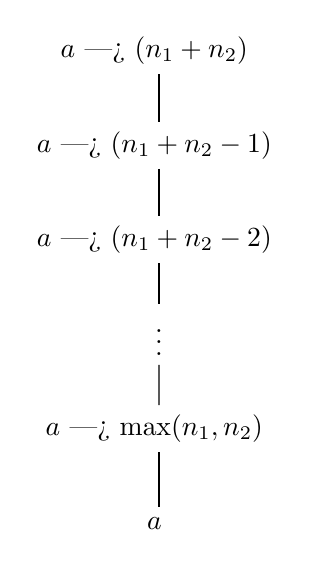
\begin{tikzpicture}[scale=0.8, every node/.style={align=center}]
            \node (Root) at (0,0) { $a$ ---> $(n_1 + n_2)$ }
                child { node { $a$ ---> $(n_1 + n_2 - 1)$ }
                    child { node { $a$ ---> $(n_1 + n_2 - 2)$ }
                        child { node {$\vdots$} 
                            child { node { $a$ ---> $\max(n_1, n_2)$ }
                                child { node { $a$ } }
                            }
                        }
                    }
                };
        \end{tikzpicture}
    \end{center}

\end{frame}

\begin{frame}
 \frametitle{Merge Function Complexity Analysis}
 \textbf{Conclusion:}  
    \[
    \text{Total Cost} \leq a(n_1 + n_2) = O(n)
    \]
\end{frame}



\begin{frame}
    \frametitle{Algorithmic Addition}
    \begin{itemize}
        \item \textbf{Problem:} \textcolor{red}{Understanding vector addition in dimension 1}
        \item Consider the number line representation:
        \begin{center}
            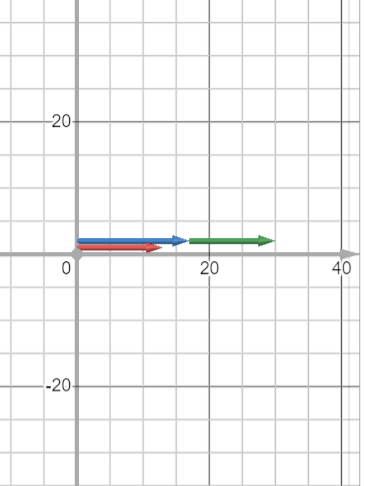
\includegraphics[width=0.4\textwidth]{figures/general/vector.png}
           
        \end{center}
    \end{itemize}
\end{frame}



\begin{frame}
\frametitle{Algorithmic Addition}
 \vspace{0.3cm}
            \textcolor{red}{$\boldsymbol{\rightarrow}$} Vector of magnitude 13\\
            \textcolor{blue}{$\boldsymbol{\rightarrow}$} Vector of magnitude 17\\
            \textcolor{green}{$\boldsymbol{\rightarrow}$} Resultant vector of magnitude 30\\
            \text Vector of magnitude 13 and 30 are of same length 
\end{frame}



\begin{frame}
    \frametitle{Example: Addition Steps}
    \begin{itemize}
        \item \textbf{Adding Numbers:} 13 + 17
        \begin{center}
            \begin{tabular}{r}
                13 \hspace{1cm} (n_1 \text{ digits})\\
                17 \hspace{1cm} (n_2 \text{ digits})\\
                \hline
                30 \hspace{1cm} \text{(with carry)}
            \end{tabular}
        \end{center}
        \vspace{0.3cm}
        \begin{itemize}
            \item Step 1: 3 + 7 = 10 (carry 1)
            \item Step 2: 1 + 1 + 1 (carried) = 3
            \item Result: 30
        \end{itemize}
    \end{itemize}
\end{frame}



\begin{frame}
    \frametitle{Important Theorem}
    \begin{itemize}
        \item \textbf{Theorem:} \textcolor{blue}{The sum of any three single-digit integers is always at most 2 digits long}
        \vspace{0.3cm}
        \item \textbf{Proof:}
        \begin{itemize}
            \item Maximum single digit is 9
            \item Maximum sum: 9 + 9 + 9 = 27
            \item Therefore, sum never exceeds 2 digits
        \end{itemize}
    \end{itemize}
\end{frame}

\begin{frame}
    \frametitle{Time Complexity Analysis}
    \begin{itemize}
        \item \textbf{Algorithm:} Add(X,Y)
        
        \vspace{0.1cm}
        \text Where |X| = n1   and |Y| = n2
        \vspace{0.3cm}
        \item \textbf{Time Complexity:} \textcolor{blue}{O(n_1 + n_2)}
        \vspace{0.1cm}
        
        \text This is a linear algorithm
        \vspace{0.3cm}
        \item \textbf{Optimality:}
        \begin{itemize}
            \item Question: Does there exist a better algorithm?
            \item Answer: No
            \item Reason: Must examine each digit at least once
             \item Mathematically: 
            \[
            E(T(n)) = \Theta(\max(n_1,n_2)) = \Theta(n_1+n_2)
            \]
        \end{itemize}
    \end{itemize}
\end{frame}


\begin{frame}
    \frametitle{Standard Multiplication Algorithm}
    \begin{itemize}
        \item Consider multiplying two numbers:
        \begin{center}
            \begin{tabular}{r}
                13 \hspace{1cm} (n_1 \text{ digits})\\
                17 \hspace{1cm} (n_2 \text{ digits})\\
                \hline
                91 \hspace{1cm} (7 \times 13)\\
                13\_ \hspace{0.8cm} (1 \times 13)\\
                \hline
                221
            \end{tabular}
        \end{center}
    \end{itemize}
\end{frame}

\begin{frame}
    \frametitle{Multiplication Time Complexity}
    \begin{itemize}
        \item \textbf{Time Complexity Analysis:}
        \begin{itemize}
            \item For each digit in n2, multiply with all digits in n1
            \item Then add the partial products
            \item Time Complexity: 
            \textcolor{blue}{O(n_1 × n_2)}

            
            \item For numbers of similar size (n1 ≈ n2 = n):
            \[
            T(n) = cn_1n_2 = \Theta(n^2)
            \]
        \end{itemize}
        \vspace{0.3cm}
        \item \textbf{Optimality Question:}
        \begin{itemize}
            \item Is this the fastest possible algorithm?
            \item Answer: \textcolor{red}{No}
            \item Reason: More efficient algorithms exist.
        \end{itemize}
    \end{itemize}
\end{frame}



\begin{frame}
    \frametitle{Summary: Asymptotic Notations}
    \begin{itemize}
        \item \textbf{Three Fundamental Rules:}
        \begin{itemize}
            \item Rule 1: Runtime bounds (Upper, Lower, Tight)
            \item Rule 2: Small inputs are irrelevant
            \item Rule 3: Constants don't matter
        \end{itemize}
        \vspace{0.3cm}
        \item \textbf{Key Points:}
        \begin{itemize}
            \item For integers: size = $\log(n)$ (bits required)
            \item Bounds valid for $n > n_0$
            \item If $T(n)$ bounded by $F(n)$, then $cT(n)$ also bounded
        \end{itemize}
    \end{itemize}
\end{frame}

\begin{frame}
    \frametitle{Summary: Quick Sort Implementations}
    \begin{block}{\textcolor{red}{Three Versions:}}
        \begin{itemize}
            \item \textbf{QS1:} Basic with rank
            \begin{itemize}
                \item $O(n^2)$ complexity
                \item Uses rank comparisons
            \end{itemize}
            \vspace{0.2cm}
            \item \textbf{QS2:} Improved with partitioning
            \begin{itemize}
                \item $O(n \log n)$ average case
                \item Extra memory for partitions
            \end{itemize}
            \vspace{0.2cm}
            \item \textbf{In-Place QS:}
            \begin{itemize}
                \item $O(1)$ extra space
                \item $O(n \log n)$ average case
                \item Randomized pivot selection
            \end{itemize}
        \end{itemize}
    \end{block}
\end{frame}

\begin{frame}
    \frametitle{Summary: Merge Sort}
    \begin{block}{Algorithm Overview}
        \begin{enumerate}
            \item Divide array into halves
            \item Recursively sort each half
            \item Merge sorted halves
        \end{enumerate}
    \end{block}
    
    \begin{alertblock}{Complexity Analysis}
        \begin{itemize}
            \item Recurrence: $T(n) = 2T(n/2) + O(n)$
            \item Final Complexity: $O(n \log n)$
            \item Merge Function: $S(n_1, n_2) = O(n_1 + n_2)$
        \end{itemize}
    \end{alertblock}
\end{frame}

\begin{frame}
    \frametitle{Summary: Elementary Operations}
    \begin{itemize}
        \item \textbf{Addition:}
        \begin{itemize}
            \item Time Complexity: $O(n_1 + n_2)$
            \item Proven optimal - must examine each digit
        \end{itemize}
        \vspace{0.3cm}
        \item \textbf{Multiplication:}
        \begin{itemize}
            \item Standard: $O(n_1 \times n_2)$            
        \end{itemize}
    \end{itemize}
\end{frame}

\begin{frame}
    \frametitle{Key Theorems and Results}
    \begin{block}{\textcolor{red}{Important Theorems:}}
        \begin{itemize}
            \item Sum of three single-digit integers $\leq$ 2 digits
            \item Randomized QS pivot expected between $\frac{n}{4}$ and $\frac{3n}{4}$
        \end{itemize}
    \end{block}
    
    \begin{alertblock}{Critical Insights}
        \begin{itemize}
            \item Quick Sort randomization improves average case
            \item Merge Sort always guarantees $O(n \log n)$
            \item Arithmetic operations can be optimized beyond naive approaches
        \end{itemize}
    \end{alertblock}
\end{frame}

